% ==============================================================
\begin{figure}[t]
    \centering
    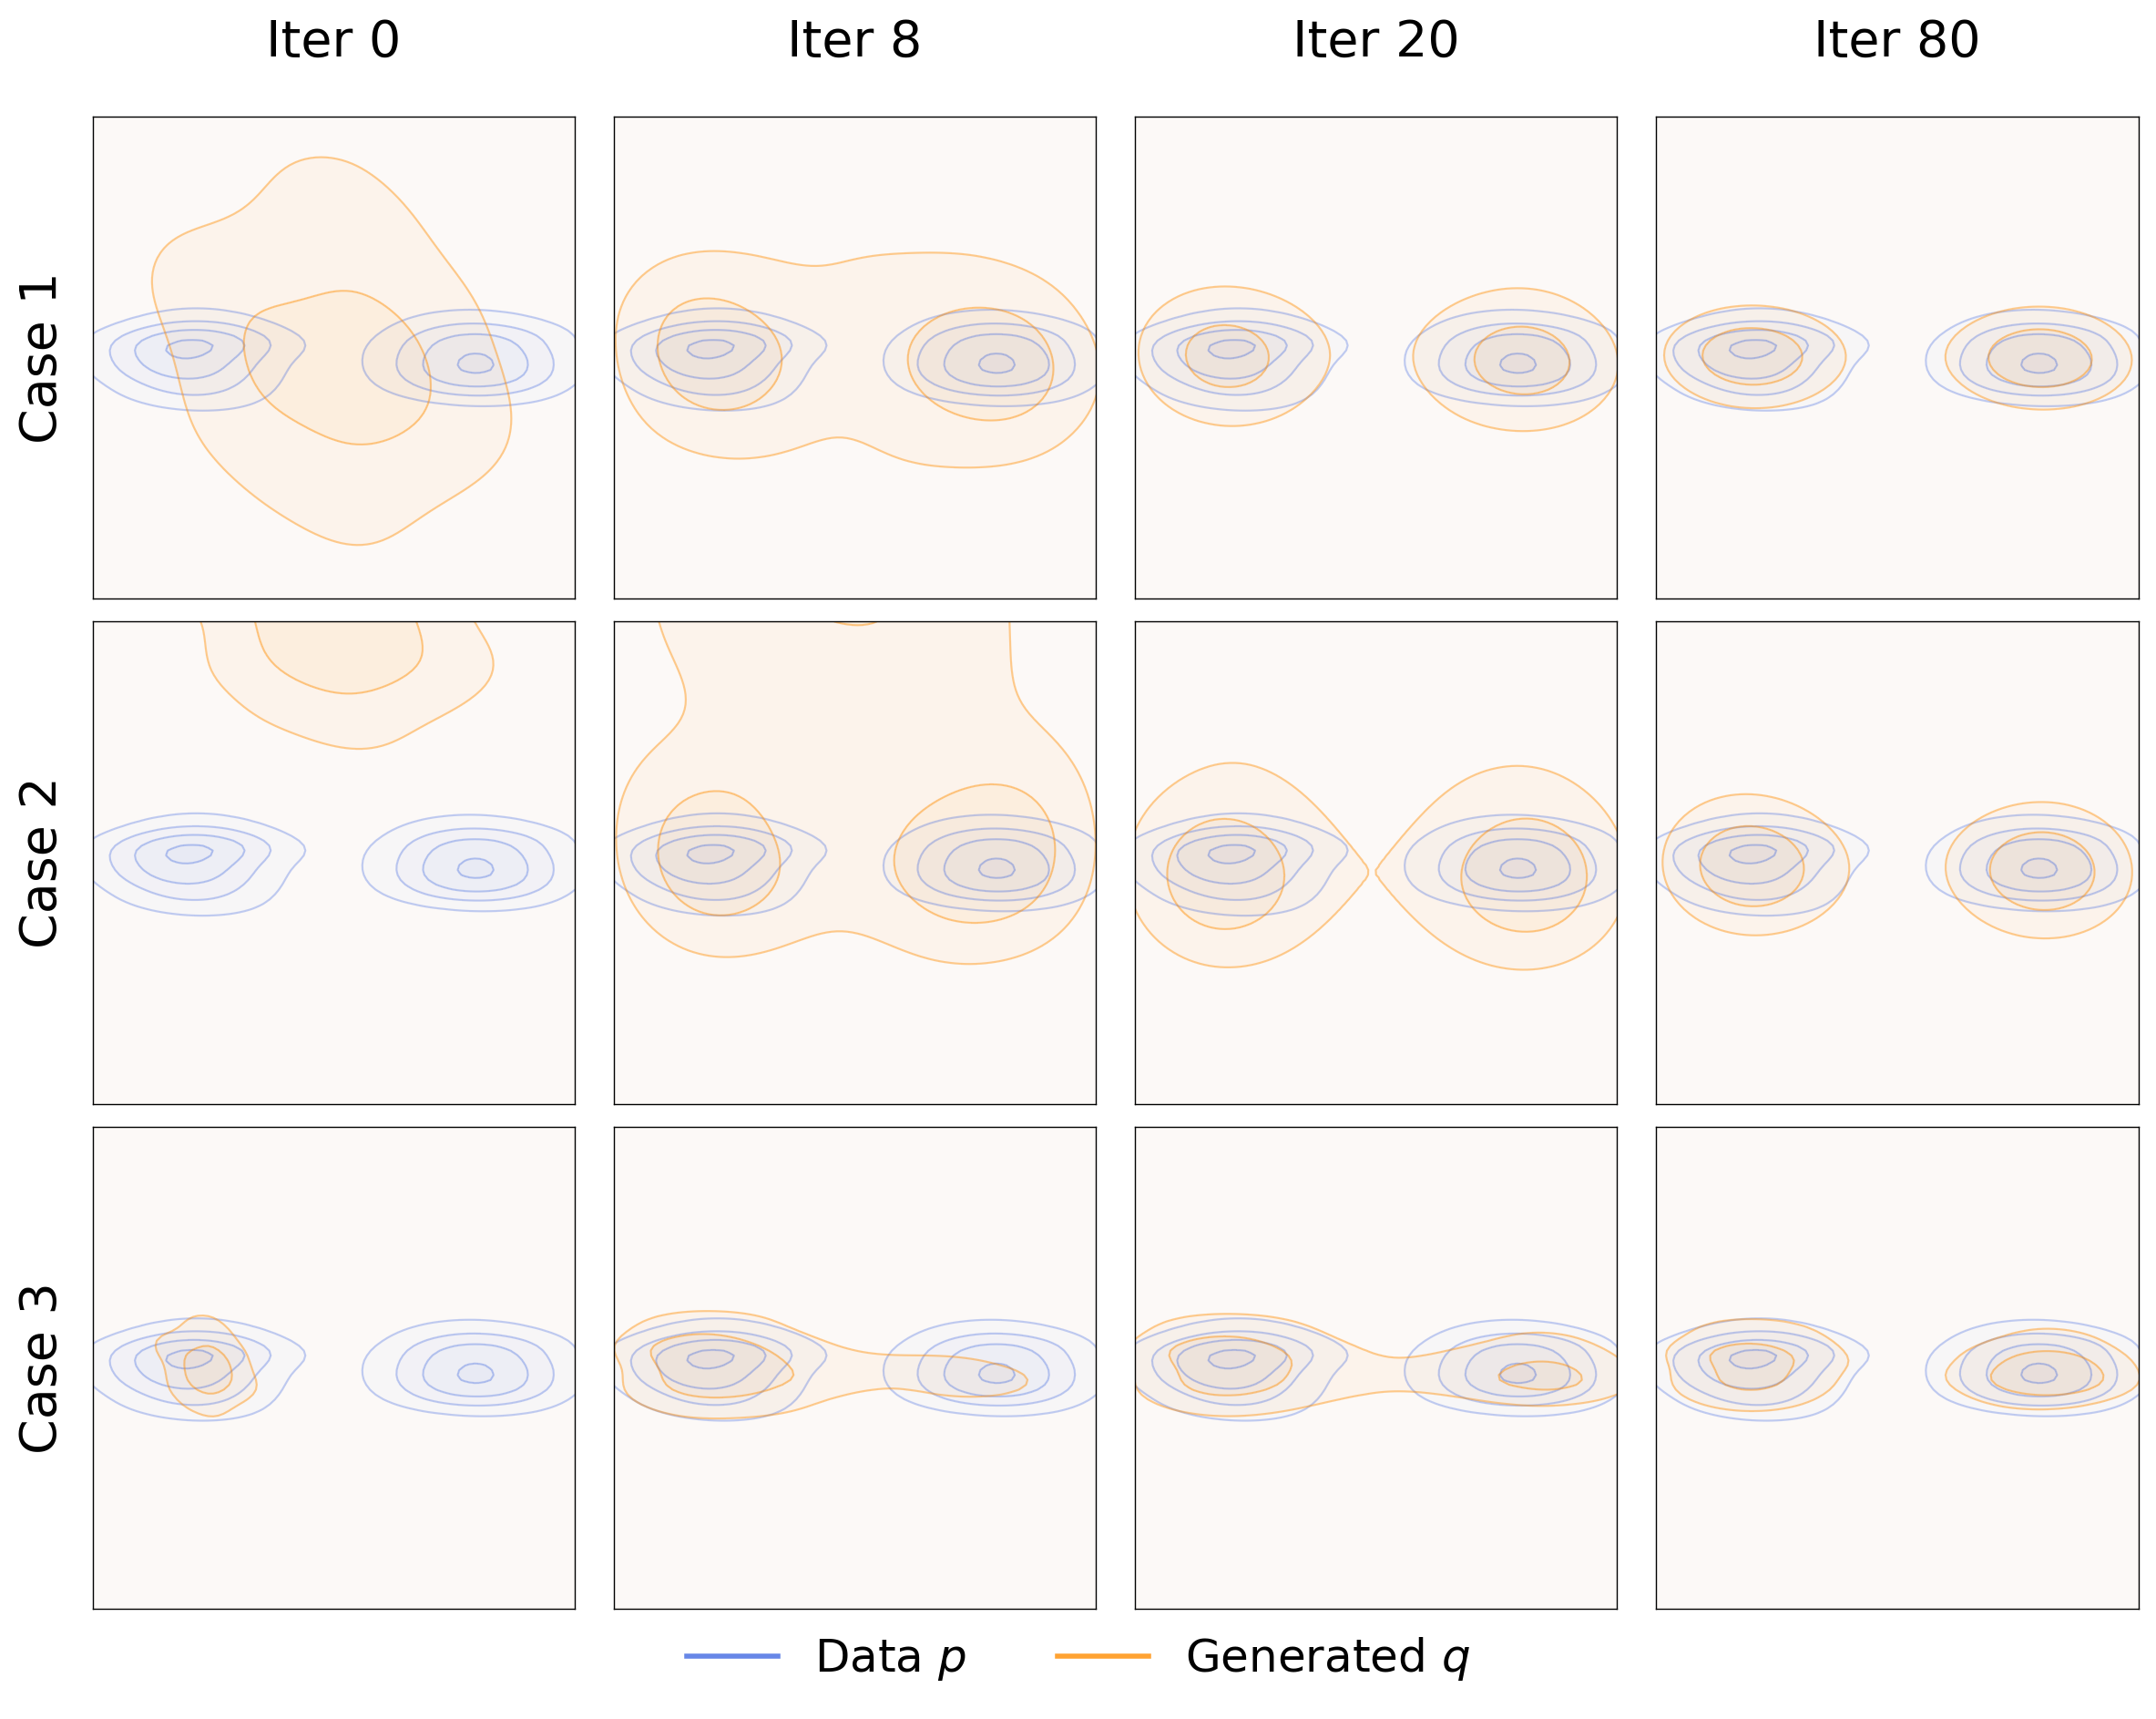
\includegraphics[width=\columnwidth]{figures/dynamics_comparison.png}
    \vspace{-1.5em}
    \caption{\textbf{Evolution of the generated distribution.}
    The distribution $q$ ({\color{orange}{orange}}) evolves toward a bimodal target $p$ ({\color{blue}{blue}}) during training. 
    We show three initializations of $q$:
    \textbf{(top)}: initialized between the two modes;
    \textbf{(middle)}: initialized far from both modes;
    \textbf{(bottom)}: initialized collapsed onto one mode.
    Across all initializations, our method approximates the target distribution without mode collapse.
    }
\label{fig:drifting_evolution_macro}
\vspace{-1em}
\end{figure}
% ==============================================================


\section{Experiments}

\subsection{Toy Experiments}

\paragraph{Evolution of the generated distribution.}
\cref{fig:drifting_evolution_macro} visualizes a 2D toy case, where $q$ evolves toward a bimodal distribution $p$ at training time, under three initializations.

In this toy example, our method approximates the target distribution without exhibiting mode collapse.
This holds even when $q$ is initialized in a collapsed single-mode state (bottom). 
This provides intuition into why our method is robust to mode collapse: 
if $q$ collapses onto one mode, other modes of $p$ will attract the samples, allowing them to continue moving and pushing $q$ to continue evolving.

% ==============================================================
\begin{figure}[t]
    \centering    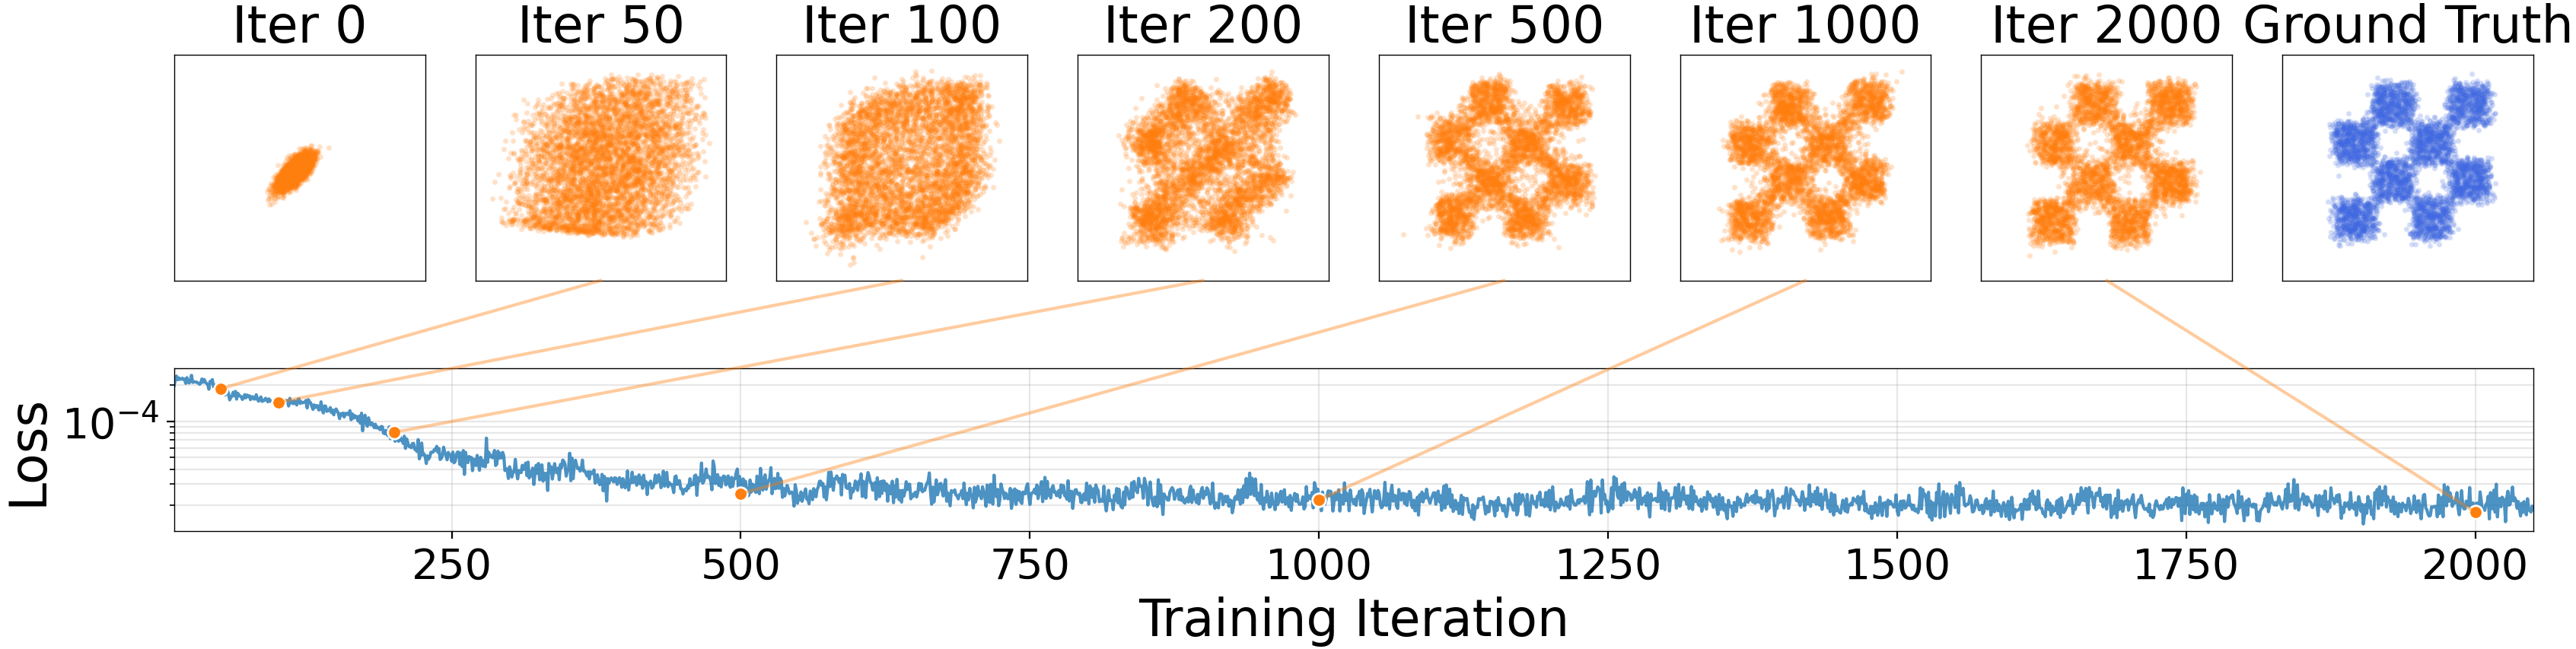
\includegraphics[width=\linewidth]{figures/toy_checkerboard_progression.png}    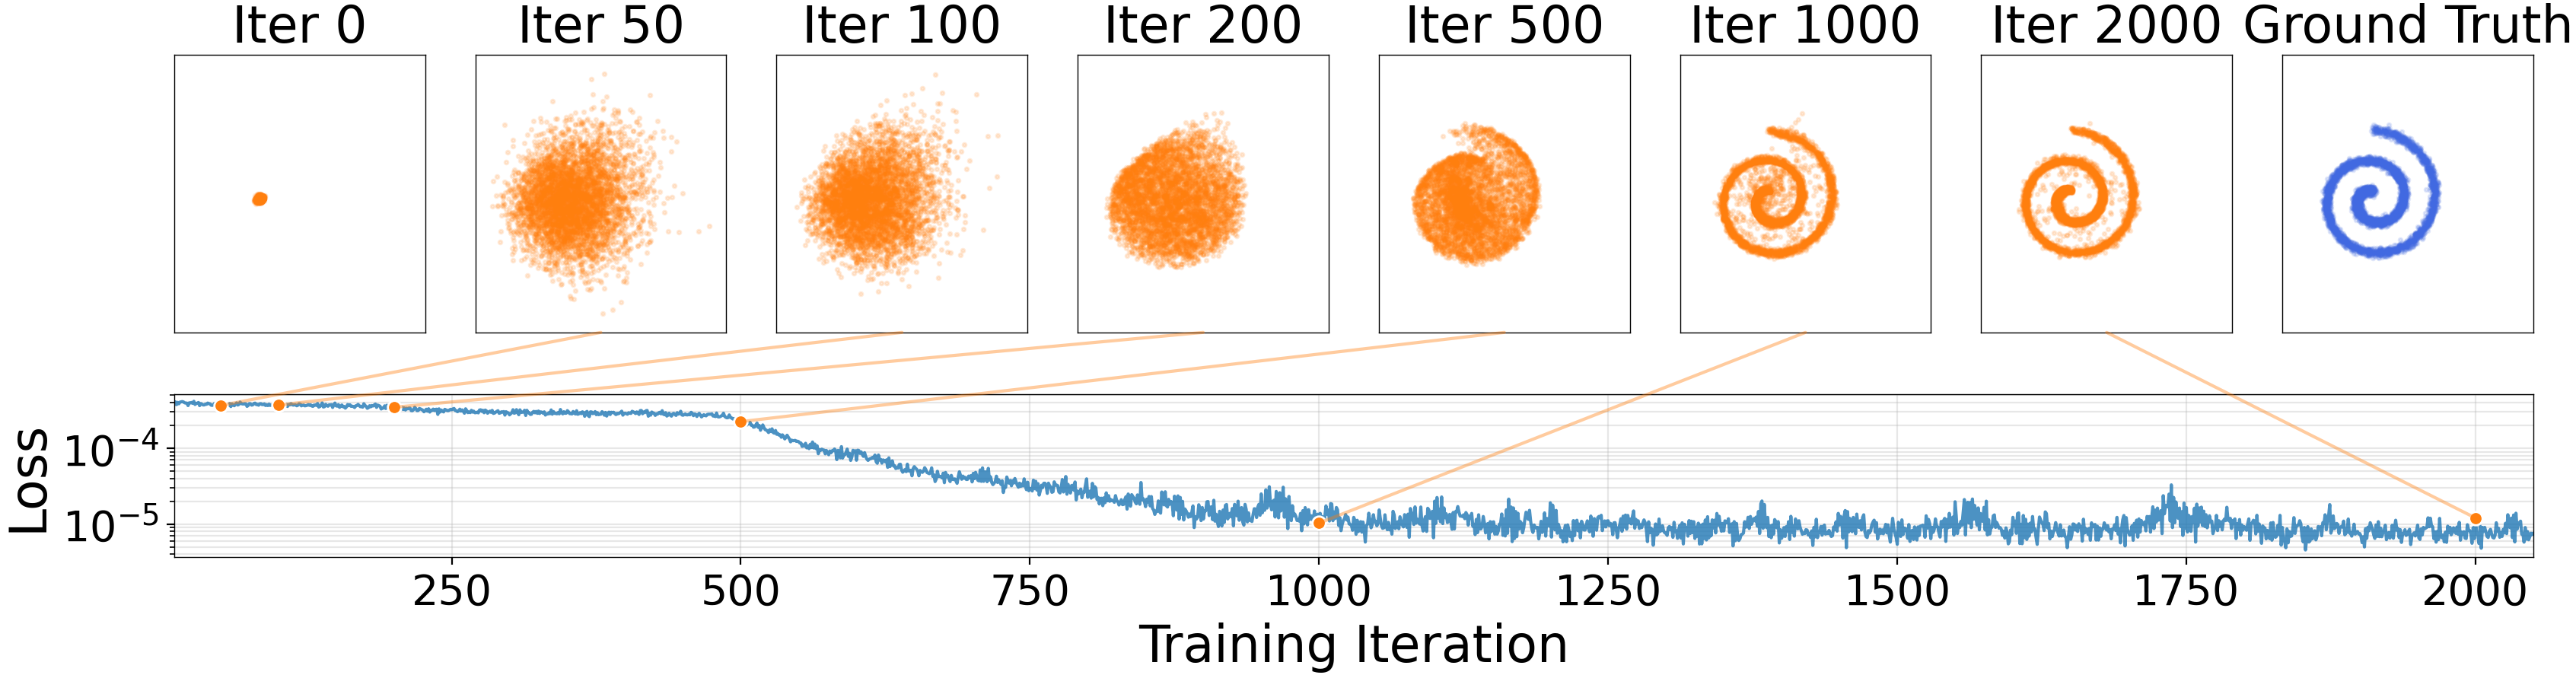
\includegraphics[width=\linewidth]{figures/toy_swiss_progression.png}
    \vspace{-.75em}
    \caption{
    \textbf{Evolution of samples.}
    We show generated points sampled at different training iterations, along with their loss values.
    The loss (whose value equals $\|V\|^2$) decreases as the distribution converges to the target. (y-axis is log-scale.)
    }
    \label{fig:toy_distributions}
\end{figure}
% ==============================================================

\paragraph{Evolution of the samples.}
\cref{fig:toy_distributions} shows the training process
on two 2D cases. A small MLP generator is trained.
The loss (whose value equals $\|\V\|^2$) decreases as the generated distribution converges to the target.
This is in line with our motivation that reducing the drift and pushing towards the equilibrium will approximately yield $p = q$.




% ###################################
\begin{table}[t]
% \vspace{-.5em}
\caption{
\textbf{Importance of anti-symmetry:}
breaking the anti-symmetry leads to failure. Here, the anti-symmetric case is defined in Eq.~(\ref{eq:V_pos_neg}) and Eq.~(\ref{eq:VZZ});
other destructive cases are defined in similar ways.
(Setting: B/2 model, 100 epochs)
}
\label{tab:ablation_antisymmetry}
% \vspace{.5em}
\tablestyle{4pt}{1.05}
\tablefontsize
\begin{tabular}{y{100}x{60}z{35}}
\toprule
case & drifting field $\V$ & FID \\
\midrule
\textbf{anti-symmetry} (default) & $\V^+ - \V^-$ & \textbf{8.46} \\
\midrule
1.5$\times$ attraction & $1.5\V^+ - \V^-$ & 41.05 \\
1.5$\times$ repulsion & $\V^+ - 1.5\V^-$ & 46.28 \\
2.0$\times$ attraction & $2\V^+ - \V^-$ & 86.16 \\
2.0$\times$ repulsion & $\V^+ - 2\V^-$ & 112.84 \\
attraction-only & $\V^+$ & 177.14 \\
\bottomrule
\end{tabular}
\end{table}
% ###################################

\subsection{ImageNet Experiments}

We evaluate our models on ImageNet 256$\times$256. Ablation studies use a B/2 model on the SD-VAE latent space, trained for 100 epochs.
The drifting loss is in a feature space computed by a latent-MAE encoder.
We report FID \cite{fid} on 50K generated images.
We analyze the results as follows.

\paragraph{Anti-symmetry.}
Our derivation of equilibrium requires the drifting field to be anti-symmetric; see Eq.~(\ref{eq:asym}). In Table~\ref{tab:ablation_antisymmetry}, we conduct a \textit{destructive} study that intentionally breaks this anti-symmetry.
The anti-symmetric case (our ablation default) works well, while other cases fail catastrophically.

Intuitively, for a sample $\x$, 
we want attraction from $p$ to be canceled by repulsion from $q$ when $p$ and $q$ match. This equilibrium is not achieved in the destructive cases.

% ###################################
\DeclareRobustCommand{\bgpos}[1]{%
  \begingroup
  \setlength{\fboxsep}{1pt}%
  \raisebox{0pt}[\height][0pt]{\colorbox{blue!15}{#1}}%
  \endgroup
}
\DeclareRobustCommand{\bgneg}[1]{%
  \begingroup
  \setlength{\fboxsep}{1pt}%
  \raisebox{0pt}[\height][0pt]{\colorbox{orange!15}{#1}}%
  \endgroup
}
\begin{table}[t]
    \centering
    \caption{
    \textbf{Allocation of positive and negative samples.}
    In both sub-tables, we control the total compute by fixing the epochs (100) and the batch size $B=N_\text{c}{\times}N_\text{pos}$ (4096). Here, $N_\text{c}$ is for class labels. Under the same budget, increasing \bgpos{positive} samples (\textbf{left}) and \bgneg{negative} samples (\textbf{right}) improves generation quality. (Setting: B/2 model, 100 epochs)
    }
    \label{tab:ablation_scaling}
    % \vspace{.5em}
    \begin{minipage}[t]{0.48\linewidth}
        \centering
        \tablestyle{2.5pt}{1.02}
        \tablefontsize
        \begin{tabular}{c >{\columncolor{blue!15}}c c | c | r}
        \toprule
        $N_\text{c}$ & {$N_\text{pos}$} & $N_\text{neg}$ & $B$ & FID  \\
        \midrule
        64 &  1 & 64 & 4096 & 20.43 \\
        64 &  16 & 64 & 4096 & 10.39 \\
        64 &  32 & 64 & 4096 & 8.97 \\
        64 &  \textbf{64} & 64 & 4096 & \textbf{8.46} \\
        \bottomrule
        \end{tabular}
    \end{minipage}
    \hfill
    \begin{minipage}[t]{0.48\linewidth}
        \centering
        \tablestyle{2.5pt}{1.02}
        \tablefontsize
        \begin{tabular}{c c >{\columncolor{orange!15}}c | c | r}
        \toprule
        $N_\text{c}$ & $N_\text{pos}$ & $N_\text{neg}$ & $B$ & FID  \\
        \midrule
        512 & 8 & 8 & 4096 & 11.82 \\
        256 & 16 & 16 & 4096 & 10.16 \\
        128 & 32 & 32 & 4096 & 9.32 \\
        64 & 64 & \textbf{64} & 4096 & \textbf{8.46} \\
        \bottomrule
        \end{tabular}
    \end{minipage}
\end{table}
% ###################################

\paragraph{Allocation of Positive and Negative Samples.}
Our method samples positive and negative examples to estimate $\V$ (see Alg.~\ref{alg:training_code}).
In Table~\ref{tab:ablation_scaling}, we study the effect of \bgpos{$N_\text{pos}$} and \bgneg{$N_\text{neg}$}, under fixed epochs and fixed batch size $B$.


Table~\ref{tab:ablation_scaling} shows that using larger $N_\text{pos}$ and $N_\text{neg}$ is beneficial. Larger sample sizes are expected to improve the accuracy of the estimated $\V$ and hence the generation quality.
This observation aligns with results in contrastive learning \cite{oord2018representation,he2020momentum,chen2020simple}, in which larger sample sets improve representation learning.

% ###################################
\begin{table}[t]
    \centering
    \caption{\textbf{Feature space for drifting.}
    We compare self-supervised learning (SSL) encoders.
    Standard SimCLR and MoCo encoders achieve competitive results, whereas our customized latent-MAE performs best and benefits from increased width and longer training.
    (Generator setting: B/2 model, 100 epochs)
    }
    \label{tab:ablation_drift_space}
    % \vspace{.5em}
    \tablestyle{3pt}{1.02}
    \tablefontsize
    \begin{tabular}{l | c c c c | r}
    \toprule
    \multicolumn{1}{c}{} & \multicolumn{4}{c}{feature encoder ($\phi$)} & \\
    \cmidrule(lr){2-5}
    \multicolumn{1}{c}{SSL method} & arch & block & width & \multicolumn{1}{c}{SSL ep.} & FID \\
    \midrule
    SimCLR & ResNet & bottleneck & 256 & 800 & 11.05 \\
    MoCo-v2 & ResNet & bottleneck & 256 & 800 & 8.41 \\
    \midrule
    latent-MAE (default) & ResNet & basic & 256 & 192 & 8.46 \\
    latent-MAE & ResNet & basic & 384 & 192 & 7.26 \\
    latent-MAE & ResNet & basic & 512 & 192 & 6.49 \\
    latent-MAE & ResNet & basic & 640 & 192 & 6.30 \\
    \midrule
    latent-MAE & ResNet & basic & 640 & 1280 & 4.28 \\
    latent-MAE + cls ft & ResNet & basic & 640 & 1280 & \textbf{3.36} \\
    \bottomrule
    \end{tabular}
\end{table}
% ###################################

\paragraph{Feature Space for Drifting.}
Our model computes the drifting loss in a feature space (Sec.~\ref{subsec:feature_space}). Table~\ref{tab:ablation_drift_space} compares the feature encoders.
Using the public pre-trained encoders from SimCLR \cite{chen2020simple} and MoCo v2 \cite{chen2020improved}, our method obtains decent results.

These standard encoders operate in the pixel domain, which requires running the VAE decoder at training.
To circumvent this, we pre-train a ResNet-style model with the MAE objective \cite{he2022masked}, directly on the latent space.
The feature space produced by this ``latent-MAE'' performs strongly (Table~\ref{tab:ablation_drift_space}). Increasing the MAE encoder width and the number of pre-training epochs both improve generation quality; fine-tuning it with a classifier (`cls ft') boosts the results further to 3.36 FID.

The comparison in Table~\ref{tab:ablation_drift_space} shows that the quality of the feature encoder plays an important role.
We hypothesize that this is because our method depends on a kernel $k(\cdot, \cdot)$ (see Eq.~(\ref{eq:kernel})) to measure sample similarity. Samples that are closer in feature space generally yield stronger drift, providing richer training signals. This goal is aligned with the motivation of self-supervised learning.
A strong feature encoder reduces the occurrence of a nearly ``flat'' kernel (\ie, $k(\cdot, \cdot)$ vanishes because all samples are far away).


On the other hand, we report that we were unable to make our method work on ImageNet without a feature encoder. In this case, the kernel may fail to effectively describe similarity, even in the presence of a latent VAE. We leave further study of this limitation for future work.

% ###################################
\begin{table}[t]
    \centering
    \caption{\textbf{From ablation to final setting.} We train our model for more epochs, adjust hyper-parameters for this regime, and use a larger model size.
    }
    % \vspace{.5em}
\label{tab:ablation_final}
    \tablestyle{6pt}{1.02}
    \tablefontsize
    \begin{tabular}{l |l r| c}
    \toprule
    case & arch & ep & FID \\
    \midrule
    (a) baseline (from Table~\ref{tab:ablation_drift_space}) & B/2 & 100 & 3.36 \\
    \midrule
    (b) longer & B/2 & 320 & 2.51 \\
    (c) longer + hyper-param. & B/2 & 1280 & 1.75 \\
    (d) larger model & L/2  & 1280 & \textbf{1.54} \\
    \bottomrule
    \end{tabular}
\end{table}
% ###################################

% ###################################
\newcommand\headspace{\hspace{.2em}}
\colorlet{mygray}{black!40}
\newcommand{\cg}{\color{mygray}}
\begin{table}[!tb]
    \centering
    \caption{\textbf{System-level comparison: ImageNet 256$\times$256 generation in {latent} space.}
    FID is on 50K images, all reported with CFG if applicable.
    The parameter numbers are ``generator + decoder''. All generators are trained from scratch (\ie, not distilled).
    }
    % \vspace{.5em}
    \label{tab:in256_latent}
    \tablestyle{2pt}{1.02}
    \tablefontsize
    \begin{tabular}{@{}l c c c r r@{}}
    \toprule
    method & space & params & NFE & FID$\downarrow$ & IS$\uparrow$ \\    \midrule
    \rowcolor[gray]{0.9} \multicolumn{6}{l}{\textit{Multi-step Diffusion/Flows}} \\
    \headspace \cg DiT-XL/2 \tiny\cite{peebles2023scalable}  & \cg \tiny SD-VAE & \cg \tiny 675M+49M & \cg \tiny 250$\times$2 & \cg 2.27 & \cg 278.2 \\
    \headspace \cg SiT-XL/2 \tiny\cite{ma2024sit} & \cg \tiny SD-VAE & \cg \tiny 675M+49M & \cg \tiny 250$\times$2 & \cg 2.06 & \cg 270.3 \\
    \headspace \cg SiT-XL/2+REPA \tiny\cite{yu2024representation}& \cg \tiny SD-VAE & \cg \tiny 675M+49M & \cg \tiny 250$\times$2 & \cg 1.42 & \cg 305.7 \\
    \headspace \cg LightningDiT-XL/2 \tiny\cite{yao2025reconstruction}& \cg \tiny VA-VAE & \cg \tiny 675M+70M & \cg \tiny 250$\times$2 & \cg 1.35 & \cg 295.3 \\
    \headspace \cg RAE+DiT$^{\text{DH}}$-XL/2 \tiny\cite{zheng2025diffusion} & \cg \tiny RAE & \cg \tiny 839M+415M & \cg \tiny 50$\times$2 & \cg \textbf{1.13} & \cg 262.6 \\
    \midrule
    \rowcolor[gray]{0.9} \multicolumn{6}{l}{\textit{Single-step Diffusion/Flows}} \\
    \headspace iCT-XL/2 \tiny\cite{song2023improved}       & \tiny SD-VAE & \tiny 675M & \tiny 1 & 34.24 & -- \\
    \headspace Shortcut-XL/2  \tiny\cite{frans2024one} & \tiny SD-VAE & \tiny 675M & \tiny 1 & 10.60 & -- \\
    \headspace MeanFlow-XL/2 \tiny\cite{geng2025mean}  & \tiny SD-VAE & \tiny 676M & \tiny 1 & 3.43 & -- \\
    \headspace AdvFlow-XL/2 \tiny\cite{lin2025adversarial} & \tiny SD-VAE & \tiny 673M & \tiny 1 & 2.38 & 284.2 \\
    \headspace iMeanFlow-XL/2 \tiny\cite{geng2025improved}    & \tiny SD-VAE & \tiny 610M & \tiny 1 & 1.72 & 282.0 \\
    \midrule
    \rowcolor[gray]{0.9} \multicolumn{6}{l}{\textit{Drifting Models}} \\
    \headspace \textbf{Drifting Model, B/2} & \tiny SD-VAE & \tiny 133M & \tiny 1 & 1.75 & 263.2 \\
    \headspace \textbf{Drifting Model, L/2} & \tiny SD-VAE & \tiny 463M & \tiny 1 & \textbf{1.54} & 258.9 \\ 
    \bottomrule
    \end{tabular}
    \vspace{-.5em}
\end{table}

% ###################################

% ###################################
% Pixel Space Table
\begin{table}[t]
    \centering
    \caption{\textbf{System-level comparison: ImageNet 256$\times$256 generation in {pixel} space.} FID is on 50K images, all reported with CFG if applicable.
    The parameter numbers are of the generator. All generators are trained from scratch (\ie, not distilled).}
    \label{tab:in256_pixel}
    % \vspace{.5em}
    \tablestyle{2pt}{1.05}
    \tablefontsize
    \begin{tabular}{@{}l c c c c r@{}}
    \toprule
    method & space & params & NFE & FID$\downarrow$ & IS$\uparrow$ \\
    \midrule
    \rowcolor[gray]{0.9} \multicolumn{6}{l}{\textit{Multi-step Diffusion/Flows}} \\
    \headspace \cg ADM-G \tiny\cite{dhariwal2021diffusion} & \cg pix & \cg 554M & \cg 250$\times$2 & \cg 4.59 & \cg 186.7 \\
    \headspace \cg SiD, UViT/2 \tiny\cite{hoogeboom2023simple} & \cg pix & \cg 2.5B & \cg 1000$\times$2 & \cg 2.44 & \cg 256.3  \\
    \headspace \cg VDM++, UViT/2 \tiny\cite{kingma2023understanding} & \cg pix & \cg 2.5B & \cg 256$\times$2 & \cg 2.12 & \cg 267.7 \\
    \headspace \cg SiD2, UViT/2 \tiny\cite{hoogeboom2024simpler} & \cg pix & \cg -- & \cg 512$\times$2 & \cg 1.73 & \cg -- \\
    \headspace \cg SiD2, UViT/1 \tiny\cite{hoogeboom2024simpler} & \cg pix & \cg -- & \cg 512$\times$2 & \cg \textbf{1.38} & \cg -- \\
    \headspace \cg JiT-G/16 \tiny\cite{li2025back} & \cg pix & \cg 2B & \cg 100$\times$2 & \cg 1.82 & \cg 292.6 \\
    \headspace \cg PixelDiT/16 \tiny\cite{yu2025pixeldit} & \cg pix & \cg 797M & \cg 200$\times$2 & \cg 1.61 & \cg 292.7 \\
    \midrule
    \rowcolor[gray]{0.9} \multicolumn{6}{l}{\textit{Single-step Diffusion/Flows}} \\
    \headspace EPG-L/16 \tiny\cite{lei2025there} & pix & 540M & 1 & 8.82 & -- \\
    \midrule
    \rowcolor[gray]{0.9} \multicolumn{6}{l}{\textit{GANs}} \\
    \headspace BigGAN \tiny\cite{brock2018large} & pix & 112M & 1 & 6.95 & 152.8 \\
    \headspace GigaGAN \tiny\cite{kang2023scaling} & pix & 569M & 1 & 3.45 & 225.5 \\
    \headspace StyleGAN-XL \tiny\cite{sauer2022stylegan} & pix & 166M & 1 & 2.30 & 265.1 \\
    \midrule
    \rowcolor[gray]{0.9} \multicolumn{6}{l}{\textit{Drifting Models}} \\
    \headspace \textbf{Drifting Model, B/16} & pix & 134M & 1 & 1.76 & 299.7 \\
    \headspace \textbf{Drifting Model, L/16} & pix & 464M & 1 & \textbf{1.61} & 307.5 \\
    \bottomrule
    \end{tabular}
    \vspace{-.5em}
\end{table}
% ###################################

\paragraph{System-level Comparisons.} In addition to the ablation setting, we train stronger variants and summarize them in Table~\ref{tab:ablation_final}.
We compare with previous methods in Table~\ref{tab:in256_latent}.

Our method achieves \textbf{1.54} FID with \textit{native} 1-NFE generation. It outperforms all previous 1-NFE methods, which are based on approximating diffusion-/flow-based trajectories.
Notably, our Base-size model competes with previous XL-size models.
Our best model (FID 1.54) uses a CFG scale of 1.0, which corresponds to ``no CFG’’ in diffusion-based methods. 
Our CFG formulation exhibits a tradeoff between FID and IS (see \ref{section:exp_cfg}), similar to standard CFG.


We provide uncurated qualitative results in Appendix~\ref{sec:appendix_qualitative_results}, Fig.~\ref{fig:latent_uncurated_samples_1}-\ref{fig:latent_uncurated_samples_4}, with CFG 1.0.
Moreover, Fig.~\ref{fig:comparison_imf_1}-\ref{fig:comparison_imf_5} show a side-by-side comparison with improved MeanFlow (iMF) \cite{geng2025improved}, a recent state-of-the-art one-step method.

\paragraph{Pixel-space Generation.} Our method can naturally work \textit{without} the latent VAE, \ie, the generator $f$ directly produces 256$\times$256$\times$3 images. The feature encoder is applied on the generated images for computing drifting loss. We adopt a configuration similar to that of the latent variant; implementation details are in Appendix \ref{sec:appendix_impl}.

Table~\ref{tab:in256_pixel} compares different pixel-space generators.
Our \textit{one-step}, \textit{pixel-space} method achieves \textbf{1.61} FID, which outperforms or competes with previous multi-step methods.
Comparing with other one-step, pixel-space methods (GANs), our method achieves 1.61 FID using only 87G FLOPs; by comparison, StyleGAN-XL produces 2.30 FID using 1574G FLOPs. 
More ablations are in \ref{section:exp_pixel_space}.

% ##################################################
\begin{table}[t]
    \centering
    \caption{\textbf{Robotics Control: Comparison with Diffusion Policy.}
    The evaluation protocol follows Diffusion Policy \citep{chi2025diffusion}.
    This table involves four single-stage tasks and two multi-stage tasks.
    ``Drifting Policy'' (ours) replaces the multi-step Diffusion Policy generator with our one-step generator.
    Success rates are reported as the average over the last 10 checkpoints.
    }
    \label{tab:robotics_combined}
    % \vspace{0.5em}
    \tablestyle{4pt}{1.0}
    \scriptsize
    % \tablefontsize
        \begin{tabular}{llcc}
            \toprule
            & & \multicolumn{1}{c}{{Diffusion Policy}} & \multicolumn{1}{c}{\textbf{Drifting Policy}} \\
            \cmidrule(lr){3-3} \cmidrule(lr){4-4}
            Task & Setting & \multicolumn{1}{c}{{NFE: 100}} & \multicolumn{1}{c}{\textbf{NFE: 1}} \\
            \midrule
            \multicolumn{4}{l}{\textit{\textbf{Single-Stage Tasks} (State \& Visual Observation)}} \\
            \midrule
            \multirow{2}{*}{Lift} & State & {0.98} & \textbf{1.00} \\
             & Visual & {\textbf{1.00}} & \textbf{1.00} \\
            \addlinespace[0.3em]
            \multirow{2}{*}{Can} & State & {0.96} & \textbf{0.98} \\
             & Visual & {0.97} & \textbf{0.99} \\
            \addlinespace[0.3em]
            \multirow{2}{*}{ToolHang} & State & {0.30} & \textbf{0.38} \\
             & Visual & {\textbf{0.73}} & 0.67 \\
            \addlinespace[0.3em]
            \multirow{2}{*}{PushT} & State & {\textbf{0.91}} & 0.86 \\
             & Visual & {0.84} & \textbf{0.86} \\
            
            \midrule
            \multicolumn{4}{l}{\textit{\textbf{Multi-Stage Tasks} (State Observation)}} \\
            \midrule
            \multirow{2}{*}{BlockPush} & Phase 1 & {0.36} & \textbf{0.56} \\
             & Phase 2 & {0.11} & \textbf{0.16} \\
            \addlinespace[0.3em]
            \multirow{4}{*}{Kitchen} & Phase 1 & {\textbf{1.00}} & \textbf{1.00} \\
             & Phase 2 & {\textbf{1.00}} & \textbf{1.00} \\
             & Phase 3 & {\textbf{1.00}} & 0.99 \\
             & Phase 4 & {\textbf{0.99}} & 0.96 \\
            \bottomrule
        \end{tabular}
        \vspace{-0.5em}
\end{table}
% ##################################################

\subsection{Experiments on Robotic Control}

Beyond image generation, we further evaluate our method on robotics control. Our experiment designs and protocols follow \textit{Diffusion Policy} \citep{chi2025diffusion}. At the core of Diffusion Policy is a multi-step, diffusion-based generator; we replace it with our one-step Drifting Model.
We directly compute drifting loss on the \textit{raw} representations for control, using no feature space. Results are in Table~\ref{tab:robotics_combined}.
Our 1-NFE model matches or exceeds the state-of-the-art Diffusion Policy that uses 100 NFE.
This comparison suggests that Drifting Models can serve as a promising generative model across different domains.




















